%%%%%%%%%%%%%%%%%%%%%%%%%%%%%%%%%%%%%%%%%%%%%%%%%%%%%%%%%%%%%%%%%%%%%%%%%%%%%%%%
\documentclass[twocolumn]{revtex4}
%%%%%%%%%%%%%%%%%%%%%%%%%%%%%%%%%%%%%%%%%%%%%%%%%%%%%%%%%%%%%%%%%%%%%%%%%%%%%%%%
% Note that comments begin with a "%" and are not turned into text in the .pdf
% document.
%%%%%%%%%%%%%%%%%%%%%%%%%%%%%%%%%%%%%%%%%%%%%%%%%%%%%%%%%%%%%%%%%%%%%%%%%%%%%%%%
% Include some extra packages.
%%%%%%%%%%%%%%%%%%%%%%%%%%%%%%%%%%%%%%%%%%%%%%%%%%%%%%%%%%%%%%%%%%%%%%%%%%%%%%%%
\usepackage[]{graphicx}
% Your abstract is a 1 paragraph summary of the project.
    %You should summarize the motivation, the procedure, and the 
    %results here
    %%%%%%%%%%%%%%%%%%%
%%%%%%%%%%%%%%%%%%%%%%%%%%%%%%%%%%%%%%%%%%%%%%%%%%%%%%%%%%%%%%%%%%%%%%%%%%%%%%%%
%%%%%%%%%%%%%%%%%%%%%%%%%%%%%%%%%%%%%%%%%%%%%%%%%%%%%%%%%%%%%%%%%%%%%%%%%%%%%%%%
\begin{document}
%%%%%%%%%%%%%%%%%%%%%%%%%%%%%%%%%%%%%%%%%%%%%%%%%%%%%%%%%%%%%%%%%%%%%%%%%%%%%%%%
\title{
Predicting the Weather
}
\author{Ben~Ellsworth}
\affiliation{Siena College, Loudonville, NY}
\date{\today}

\begin{abstract}
This assignment was assigned as a final project in order to test our knowledge of python, very specifically in doing Monte Carlo simulations. In this project I used given chances of rain to calculate the probability of rain on a given amount of days per month, and then to calculate the amount of rainfall in a month. Using Monte Carlo simulations, I found that when there is a 20\% chance of rain, it is more likely to rain on one and only one day in a month as opposed to raining 8 days in a month where the chance of rain on a given day was 10\%. These problems would be very difficult to do with pen and paper, which is why we are using this approach. I also used this method to calculate the average rainfall in a month with specific conditions that influence how much rain and how likely it is to rain, and found the average rainfall in a given month to be about 8.1cm. 
\end{abstract}

\maketitle
%%%%%%%%%%%%%%%%%%%%%%%%%%%%%%%%%%%%%%%%%%%%%%%%%%%%%%%%%%%%%%%%%%%%%%%%%%%%%%%%

%%%%%%%%%%%%%%%%%%%%%%%%%%%%%%%%%%%%%%%%%%%%%%%%%%%%%%%%%%%%%%%%%%%%%%%%%%%%%%%%
\section{Introduction}
The purpose of this analysis was to apply our programming skills, particularly in doing a Monte Carlo simulation, to predict the weather. We are given the chance of it raining on a day, and then use this information compared to a randomly generated number. If the random number falls within a certain range(derived from the probability), then it does in fact rain. When repeated over a large number of trials, this actually gives a very accurate representation of what would happen. 

%%%%%%%%%%%%%%%%%%%%%%%%%%%%%%%%%%%%%%%%%%%%%%%%%%%%%%%%%%%%%%%%%%%%%%%%%%%%%%%%

%%%%%%%%%%%%%%%%%%%%%%%%%%%%%%%%%%%%%%%%%%%%%%%%%%%%%%%%%%%%%%%%%%%%%%%%%%%%%%%%
\section{Problem I}
For the first problem, we are given that there is a {\bf20\%} of it raining on any given day in a month, then asked to calculate the chances of it raining on one and only one day in a month. First, we must work this problem out analytically. You want to figure out the chances it rains on {\bf one and only one} day of the month. This means it can rain on the first day, and not the rest. {\it OR} it could rain on the second day, and not the rest, and so on. To do this, you first calculate the chances of it raining on one day, which would be \underline{$.20 * .80^{29}$}. The .20 represents the chance of rain, multiplied by one day, and the {$.80^{29}$} includes the other 29 days of no rain. Regardless of whether it rains on the first or last day, you will be doing the same equation. Therefore, you can multiply \underline{$30 * .20 * .80^{29}$} to get the total probability of it raining once in an entire month, on any of the given 30 days. This comes out to be a {\bf.928\%} probability of it raining on only one day in a month.\\
    Next we do this problem using a Monte Carlo approach. To do this, I write a function that does the following 30 times, to simulate an entire month: generates a random number between 0 and 1, and if this number falls between 0 and .20 (the odds of it raining), then it rains! Then, since it rains we add 1 to a counter. After going through this 30 times, if the counter is equal to 1, that means we have a month where it rained only one day. If the counter does not equal 1, then we do nothing. This is then run through a loop of 10,000 months, and the total number of months with it raining one and only one day is divided by the total number of months, then multiplied by 100. The final calculation is {\bf.923\%}, coming quite close to the analytical approach, and justifying this method. 

\section{Problem II}
The next problem asks us to do a similar thing, using only a Monte Carlo approach. We are given that the chance of rain on a given day is {\bf10\%}, and we want to know the probability that it rains on {\it at least} 8 days in a month, and it can be {\it any} combination of 8 days. To solve this problem I took a very similar approach to the previous one. I generated a random number between 0 and 1, and if this number was between 0 and .10 I added 1 to a counter. After a 30 day loop, if the total of the counter was {\it greater than or equal to 8}, that signified a month in which it rained 8 or more days. I then ran this function 10,000 times, and counted the number of months in which it rained 8 or more days, and divided by the total number of months, and finally multiplied by 100 to get a percent. My finding for this problem was that there is about a {\bf.79\%} chance of it raining any 8 days in a given month. 
\section{Problem III}
\subsection{}
The third problem is a bit more complex. We are asked to calculate the probability of it raining more than 10cm in a given month. We are given that the chances of it raining on a day are: 
\begin{itemize}
\item If it is the first day of the month, there is a 10\% chance of rain.
\item If it rained 1 day before, but not 2 days before, there is a 20\% chance of rain. 
\item If it rained both of the 2 days before, but not the 3rd day before, there is a 25\% chance of rain.
\item If it rained for the 3 days (or more) before, there is a 5\% chance of rain.  
\item Otherwise, there is a 10\% chance of rain.
\end{itemize}
We are also given the chances of certain amounts of~rain, if it does indeed rain.
\begin{center}
\begin{tabular}{c | c} 
Amount of rain (cm) & Chance(\%) \\
\hline
1 & 20 \\
2 & 30 \\
3 & 30 \\
4 & 10 \\
5 & 10 \\
\end{tabular}
\end{center}
To approach this problem, I first make a function. This function runs 1 month at a time, and generates a random number between 0 and 1. Then, I set conditions for the days. For example, if it is the first day, then the chance of rain is 10\%. So, if day=1, and the random number falls in between 0 and .10, then it rains. For the second "day condition", if day is greater than 2, and day-1=True, and day-2=False, then there is a 20\% chance of rain. Therefore, if the random number is between 0 and .20, then it rains. This process continues through each "day condition" with a nested conditional. The "day condition" figures out what the chance of rain is based on the conditions given, and then within that, since the chance of rain is determined, the random number is compared to see whether it rains or not.\\
Within the function, there is another section. If it does rain, another random number between 0 and 1 is generated. I then use the given chances for the amount of rain, and compare it to this random number. For example, there is a 20\% chance that it rains one cm. If the random number is between 0 and .20, then it rains one cm. There's a 30\% chance that it rains 2 cm, so if the random number is between .20 and .50, then it rains 2cm. I continue this, using the last part of the previous range for my starting point, up to 1.\\
This entire function is run in a loop of 100,000 months, and every time the rainfall is greater than 10cm, it adds one to a counter. The total of that counter is divided by the number of months and multiplied by 100 to get a percentage, which comes out to about 35\%, meaning it rains at least 10cm in a given month 35\% of the time. 
\subsection{}
To create a histogram of rainfall values, I created a loop that ran my function of calculating the amount of rain 100,000 times. Outside of the function I defined a variable as an empty set, and every time through the loop I appended the empty set to store all my rainfall values. Then, using matplotlib, I plotted the rainfall and labeled my axes.
\begin{figure}[h]
\centering
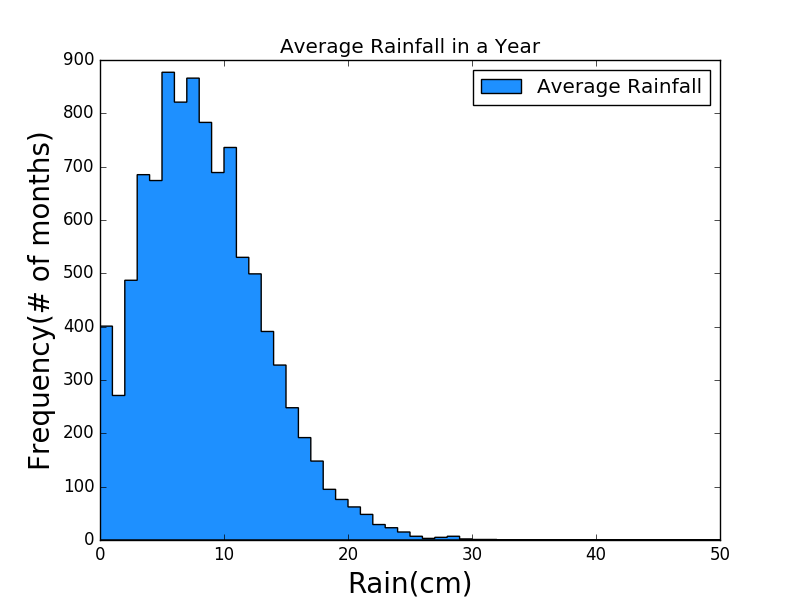
\includegraphics[width=0.35\textwidth]{avg_rain_graph.png}
\caption{Rainfall distribution}
\end{figure}
\subsection{}
To calculate the average rainfall in a given month, I used another loop. I defined a total of 0 outside of the loop, to add the rainfall values to. I used the range(0, nmonths), and each time through the loop I added the rainfall to the total. This gave me a sum of all of the rainfall. Then outside the loop, I divided this total by nmonths, which was 100,000 again in this case, to get an average, which came out to be roughly 8.1cm per month.
\subsection{}
In order to calculate the range of rainfall values, I used python to eliminate the first 2.5\% and the last 2.5\%. I did this by using a {\it sort} function that sorted my list of rainfall values. I then defined a variable called remove as an empty set. I looped over the first 250 values of the sorted rainfall, and appended them to the list remove. I then did the same thing for the last 250 values. Then, I compared the the original list to the "remove" list, to determine my range. Therefore, I am able to say that I am 95\% confident that it will rain between 0cm and 19cm in a given month. 
%%%%%%%%%%%%%%%%%%%%%%%%%%%%%%%%%%%%%%%%%%%%%%%%%%%%%%%%%%%%%%%%%%%%%%%%%%%%%%%%

%%%%%%%%%%%%%%%%%%%%%%%%%%%%%%%%%%%%%%%%%%%%%%%%%%%%%%%%%%%%%%%%%%%%%%%%%%%%%%%%
\end{document}
%%%%%%%%%%%%%%%%%%%%%%%%%%%%%%%%%%%%%%%%%%%%%%%%%%%%%%%%%%%%%%%%%%%%%%%%%%%%%%%%
